\documentclass[11pt, oneside]{article} 
\usepackage{geometry}
\geometry{letterpaper} 
\usepackage{graphicx}
	
\usepackage{amssymb}
\usepackage{amsmath}
\usepackage{parskip}
\usepackage{color}
\usepackage{hyperref}

\graphicspath{{/Users/telliott/Github/calculus_book/png/}}
% \begin{center} 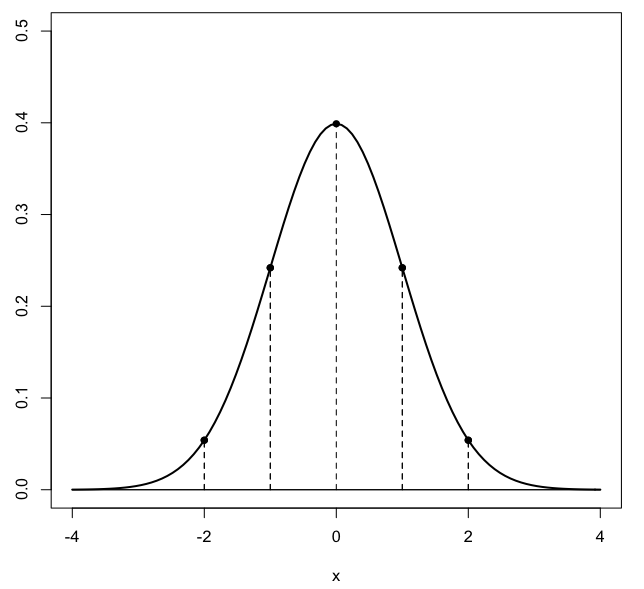
\includegraphics [scale=0.4] {gauss3.png} \end{center}

\title{Circles}
\date{}

\begin{document}
\maketitle
\Large
From a previous chapter, Euclid's third postulate was:

$\circ$   Given any straight line segment, a circle can be drawn having the segment as radius and one endpoint as center.  The tool to do this is a compass.

If the radius is extended so that it cuts the circle at two points, it is called a diameter.  

We saw previously that one can construct a line perpendicular to any given line.  If that line is constructed perpendicular to the diameter at the point where it meets the circle, the new line is called a tangent line.  By definition, the tangent line touches the circle at a single point.

\subsection*{arcs of a circle}

\begin{center} 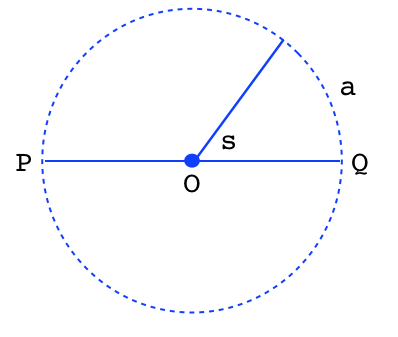
\includegraphics [scale=0.4] {arcs11.png} \end{center}

In calculus and analytical geometry angles are defined in terms of radians of arc. In the figure above, the angle $s$ is \emph{defined to be equal to} the length of arc $a$ that it sweeps out, or subtends in a unit circle.

For a unit circle with radius = $1$, the total circumference is $2\pi$, so the arc swept out by the angle $\theta$, measured in radians, is in the same ratio to $2 \pi$ as the ratio of the angle's measure in degrees to $360^\circ$.

It seems natural then to adopt the arc length as a measure of the angle, where $360^\circ$ is equal to $2 \pi$ \emph{radians}, and an angle of $90^\circ$, for example, a right angle, is equal to $\pi/2$ radians.

\begin{center} 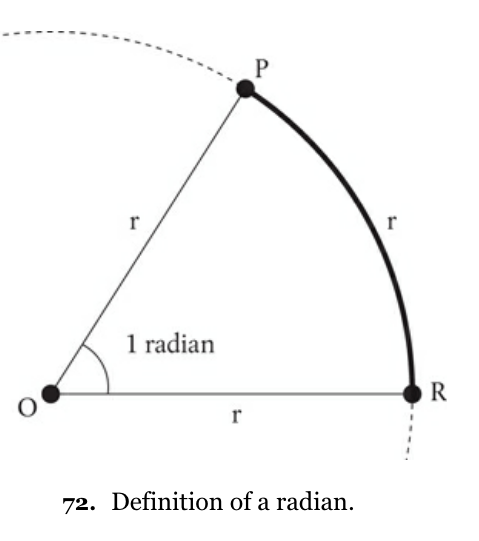
\includegraphics [scale=0.30] {radian.png} \end{center}

One can easily divide $360$ by $2 \pi$ to find that one radian is approximately $57^\circ$.
  
To convert some more measures of angles in degrees to radians:
\[ 180^\circ = \pi, \ 90^\circ = \frac{\pi}{2} \]
\[ 60^\circ = \frac{\pi}{3}, \ 45^\circ = \frac{\pi}{4}, \ 30^\circ = \frac{\pi}{6} \]

Central angle and subtended arc are numerically equal, but remember that they are dimensionally different.  Arc is a length, angle is just an angle.

\subsection*{Thales' theorem}

In this chapter, we introduce a few more theorems concerning circles, starting with the last of Thales' theorems:

$\circ$  Any angle inscribed in a semicircle is a right angle.

Think of three points on the circumference of the circle as forming a triangle. If two points are on a diameter of the circle, the angle formed at any arbitrary but distinct third point is always a right angle.

To prove: $\angle PRQ$ is a right angle.
\begin{center} 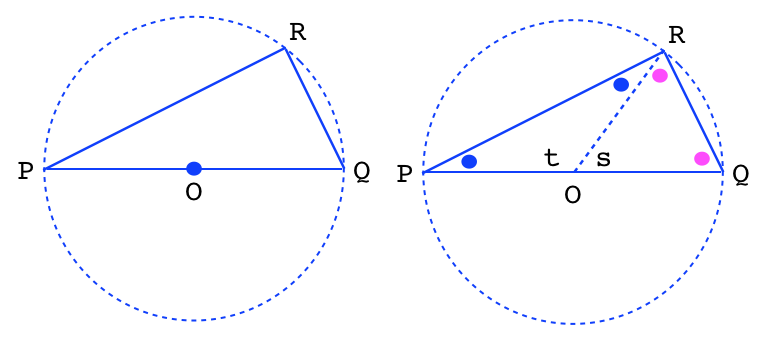
\includegraphics [scale=0.4] {arcs12.png} \end{center}

Solution:

Draw the radius OR. Notice that the two smaller triangles produced ($\triangle OPR$ and $\triangle OQR$) are both isosceles, since two of their sides are radii of the circle.

Therefore, in each triangle the two angles marked with dots of the same color are equal  (by P $I.5$).

Since $\angle PRQ$ contains one angle of each type, it is equal to one-half the angle sum for the triangle, i.e., $\angle PRQ$ is a right angle.

\begin{center} 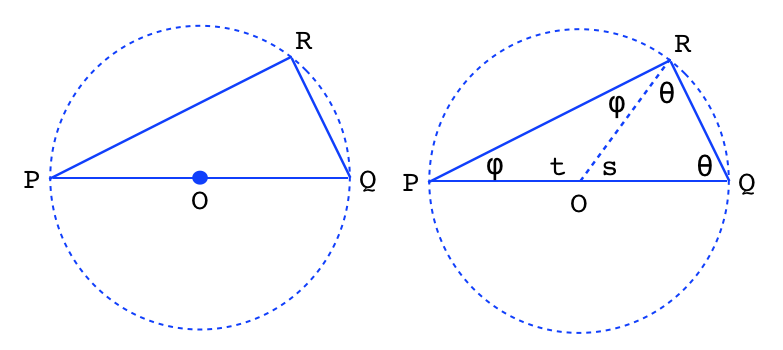
\includegraphics [scale=0.4] {arcs13.png} \end{center}

To restate this:  in the figure above, $\angle PRQ = \phi + \theta$.  Since the full measure of the triangle is $180^\circ = \pi$ radians, and
\[ \phi + \phi + \theta + \theta = \pi \]
it follows that
\[ \phi + \theta = \pi/2 \]

$\square$

\subsection*{angles on the perimeter}

The arc swept out by the right angle $\angle PRQ$ is clearly equal to $\pi$, because that arc is one-half of a circle.  

But the angles on the perimeter of the circle subtending the very same arc add up to
\[ \angle PRQ = \phi + \theta = \pi/2 \]

What's going on?

To clarify, let us label the arcs on the circle.  $a$ is the arc swept out by angle $t$, and $a$ and $t$ have the same measure by definition, although one is a length and the other an angle.

\[ t = a \]

By the external angle theorem, we know that
\[ t = 2 \theta \]
and so conclude that
\[ 2 \theta = a \]

The angle $\theta$ lying on the perimeter sweeps out the same arc as $t$, even though $\theta$ is one-half of $t$.

Apparently, since $\theta$ is farther away from the arc, its angular measure allows the arc to get bigger.

The arc length swept out by an angle on the perimeter is twice the angle's measure in radians.

\subsection*{tangent}

Consider the chord PR and draw the tangent at P.
\begin{center} 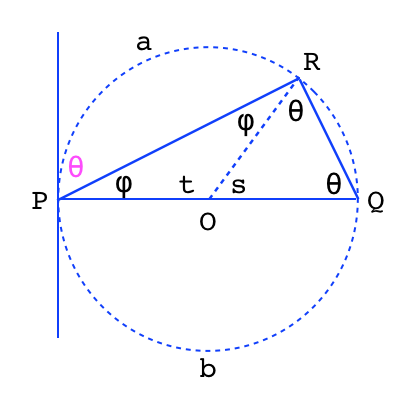
\includegraphics [scale=0.4] {arcs27.png} \end{center}

The angle between the tangent and the chord equals $\theta$ because $\theta + \phi$ is a right angle

Take a chord of the circle, draw the diameter and the tangent.
The same rule applies to both angles: one between the chord and the diameter, and the second between the chord and the tangent. The arc is twice the measure of the angle.

\subsection*{geometric mean}

We showed in the chapter on the Pythagorean theorem that the altitude of a right triangle is the geometric mean of the two components of the base.

\[ h^2 = pq \]
\[ h = \sqrt{pq} \]

According to wikipedia:

\url{https://en.wikipedia.org/wiki/Geometric_mean}

The fundamental property of the geometric mean is that (letting $m$ be the \emph{geometric mean} here):
\[ m \ [ \ \frac{x_i}{y_i} \ ] \ = \frac{m(x_i)}{m(y_i)} \]

and one consequence is that

\begin{quote}This makes the geometric mean the only correct mean when averaging normalized results; that is, results that are presented as ratios to reference values.\end{quote}

A number of examples are given in the article.

This section is here because originally, there was a proof-without-words that the geometric mean is always less than or equal to the arithmetic mean.

\begin{center} 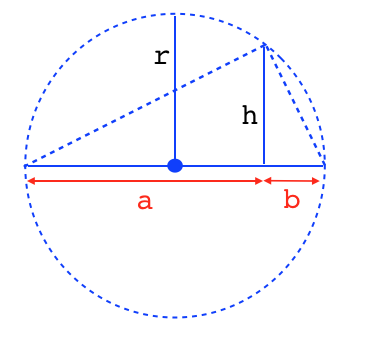
\includegraphics [scale=0.5] {geometric_mean2.png} \end{center}

I decided to use a different diagram and add some words.  A right triangle is inscribed in a semicircle.  As just mentioned, the altitude $h$ squared is equal to the product of chord segments (we will prove this geometrically in the next chapter as well).
\[ h^2 = ab \]
\[ h = \sqrt{ab} \]

But we also have that $a + b = 2r$ and hence
\[ r = \frac{a + b}{2} \]
Do you recognize these?  The second expression is the arithmetic mean of $a$ and $b$, while the first is the geometric mean.

The geometry shows that $h \le r$ so:
\[ \sqrt{ab} \le \frac{a + b}{2} \]

The geometric mean is always less than the arithmetic mean, except when $a = b$, when they are equal (or all of $n$ values are equal).

\subsection*{tangents}
Thales theorem provides a way to construct the tangent to a circle passing through any exterior point $P$.
\begin{center} 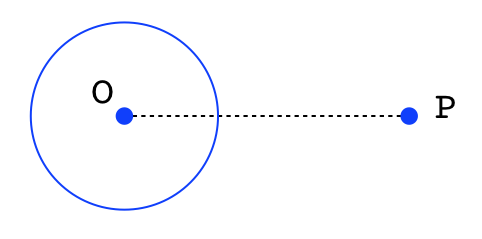
\includegraphics [scale=0.5] {tangent1.png} \end{center}
Use OP as the diameter of a circle.  Draw the line segment $OP$ and divide it in half by erecting the perpendicular bisector.  Use that distance as the radius of a new circle.  The point $R$ is the intersection of the two circles.
\begin{center} 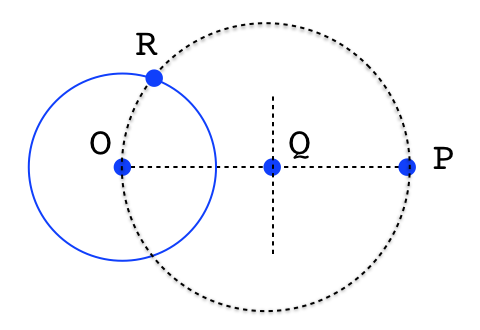
\includegraphics [scale=0.5] {tangent2.png} \end{center}

By Thales theorem, $\angle ORQ$ is a right angle, and since $OR$ is a radius of the original circle, $RQ$ is the tangent at the point $R$.

To construct a tangent on a circle at a given point $P$
\begin{center} 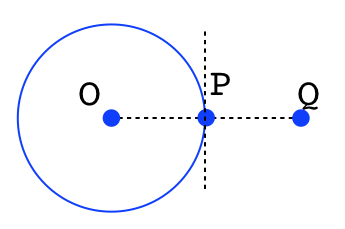
\includegraphics [scale=0.5] {tangent3.png} \end{center}
Extend $OP$ to $Q$ such that $OP$ is equal to $PQ$.  Construct the perpendicular bisector at $P$.  That is the tangent of the circle.

\end{document}